\documentclass[9pt,twocolumn,twoside,]{pnas-new}

% Use the lineno option to display guide line numbers if required.
% Note that the use of elements such as single-column equations
% may affect the guide line number alignment.


\usepackage[T1]{fontenc}
\usepackage[utf8]{inputenc}

% tightlist command for lists without linebreak
\providecommand{\tightlist}{%
  \setlength{\itemsep}{0pt}\setlength{\parskip}{0pt}}


% Pandoc citation processing
%From Pandoc 3.1.8
% definitions for citeproc citations
\NewDocumentCommand\citeproctext{}{}
\NewDocumentCommand\citeproc{mm}{%
  \begingroup\def\citeproctext{#2}\cite{#1}\endgroup}
\makeatletter
 % allow citations to break across lines
 \let\@cite@ofmt\@firstofone
 % avoid brackets around text for \cite:
 \def\@biblabel#1{}
 \def\@cite#1#2{{#1\if@tempswa , #2\fi}}
\makeatother
\newlength{\cslhangindent}
\setlength{\cslhangindent}{1.5em}
\newlength{\csllabelwidth}
\setlength{\csllabelwidth}{3em}
\newenvironment{CSLReferences}[2] % #1 hanging-indent, #2 entry-spacing
 {\begin{list}{}{%
  \setlength{\itemindent}{0pt}
  \setlength{\leftmargin}{0pt}
  \setlength{\parsep}{0pt}
  % turn on hanging indent if param 1 is 1
  \ifodd #1
   \setlength{\leftmargin}{\cslhangindent}
   \setlength{\itemindent}{-1\cslhangindent}
  \fi
  % set entry spacing
  \setlength{\itemsep}{#2\baselineskip}}}
 {\end{list}}
\usepackage{calc}
\newcommand{\CSLBlock}[1]{#1\hfill\break}
\newcommand{\CSLLeftMargin}[1]{\parbox[t]{\csllabelwidth}{#1}}
\newcommand{\CSLRightInline}[1]{\parbox[t]{\linewidth - \csllabelwidth}{#1}\break}
\newcommand{\CSLIndent}[1]{\hspace{\cslhangindent}#1}


\templatetype{pnasresearcharticle}  % Choose template

\title{Rapport - Article scientifique}

\author[a,1,4]{Marika Roberge}
\author[a,2,4]{Bertrand Labrecque}
\author[a,3,4]{Juliette Boulet-Thomas}

  \affil[a]{Faculté des sciences, Département de biologie, 2500
Boulevard de l'Université, Sherbrooke, Québec, Zip}


% Please give the surname of the lead author for the running footer
\leadauthor{Roberge}

% Please add here a significance statement to explain the relevance of your work
\significancestatement{Authors must submit a 120-word maximum statement
about the significance of their research paper written at a level
understandable to an undergraduate educated scientist outside their
field of speciality. The primary goal of the Significance Statement is
to explain the relevance of the work in broad context to a broad
readership. The Significance Statement appears in the paper itself and
is required for all research papers.}


\authorcontributions{Please provide details of author contributions
here.}

\authordeclaration{Please declare any conflict of interest here.}

\equalauthors{\textsuperscript{4} M.R.(Author One), B.L. (Author Two)
and J.B-T. (Author Three) contributed equally to this work (remove if
not applicable).}

\correspondingauthor{\textsuperscript{1} To whom correspondence should
be addressed. E-mail:
\href{mailto:marikaroberge@email.com}{\nolinkurl{marikaroberge@email.com}}}

% Keywords are not mandatory, but authors are strongly encouraged to provide them. If provided, please include two to five keywords, separated by the pipe symbol, e.g:
 \keywords{  lepidopteres |  communautés |  variation
temporelle |  variation spatiale  } 

\begin{abstract}
Please provide an abstract of no more than 250 words in a single
paragraph. Abstracts should explain to the general reader the major
contributions of the article. References in the abstract must be cited
in full within the abstract itself and cited in the text.
\end{abstract}

\dates{This manuscript was compiled on \today}
\doi{\url{www.pnas.org/cgi/doi/10.1073/pnas.XXXXXXXXXX}}

\begin{document}

% Optional adjustment to line up main text (after abstract) of first page with line numbers, when using both lineno and twocolumn options.
% You should only change this length when you've finalised the article contents.
\verticaladjustment{-2pt}



\maketitle
\thispagestyle{firststyle}
\ifthenelse{\boolean{shortarticle}}{\ifthenelse{\boolean{singlecolumn}}{\abscontentformatted}{\abscontent}}{}

% If your first paragraph (i.e. with the \dropcap) contains a list environment (quote, quotation, theorem, definition, enumerate, itemize...), the line after the list may have some extra indentation. If this is the case, add \parshape=0 to the end of the list environment.

\acknow{Please include your acknowledgments here, set in a single
paragraph. Please do not include any acknowledgments in the Supporting
Information, or anywhere else in the manuscript.}

Le rapport doit contenir :

3 figures Un titre et un résumé Une courte introduction spécifiant les
questions Une courte description de la méthode et des résultats Une
discussion, enrichie de citations provenant de la littérature
scientifique Références interne aux figures et à la bibliographie
L'ensemble du texte doit faire 1000-1500 mots max Une bibliographie

\subsection{Nos questions de
recherche}\label{nos-questions-de-recherche}

\subsubsection{\texorpdfstring{\textbf{Question principale}
:}{Question principale :}}\label{question-principale}

Quels sont les changements dans la biodiversité des espèces de
lépidoptères dans le temps et dans l'espace au Québec ?

\#\#\#Questions spécifiques (1 sur la variation temporelle et 2 sur la
variation temporelle+spatiale) : \#\#\# \textbf{Variation temporelle} :
Analyse 1 : Comment la diversité des espèces de lépidoptères a-t-elle
évoluée au fil des années?

\#\#\#\textbf{Variation temporelle et spatiale} : Analyse 2 : Comment la
dviersité et la répartition des espèces de lépidoptères a-t-elle évoluée
au fil des années? Analyse 3 : Comment la répartition de Papilio
canadensis change dans le temps et l'espace?

Please start your introduction without including the word
``Introduction'' as a section heading; this heading is implied in the
first paragraphs.

\section*{Guide to using this
template}\label{guide-to-using-this-template}
\addcontentsline{toc}{section}{Guide to using this template}

\subsection*{Author Affiliations}\label{author-affiliations}
\addcontentsline{toc}{subsection}{Author Affiliations}

Include department, institution, and complete address, with the
ZIP/postal code, for each author. Use lower case letters to match
authors with institutions, as shown in the example. Authors with an
ORCID ID may supply this information at submission.

\subsection*{Submitting Manuscripts}\label{submitting-manuscripts}
\addcontentsline{toc}{subsection}{Submitting Manuscripts}

\subsection*{Format}\label{format}
\addcontentsline{toc}{subsection}{Format}

Many authors find it useful to organize their manuscripts with the
following order of sections; Title, Author Affiliation, Keywords,
Abstract, Significance Statement, Results, Discussion, Materials and
methods, Acknowledgments, and References. Other orders and headings are
permitted.

\subsection*{Manuscript Length}\label{manuscript-length}
\addcontentsline{toc}{subsection}{Manuscript Length}

PNAS generally uses a two-column format averaging 67 characters,
including spaces, per line. The maximum length of a Direct Submission
research article is six pages and a PNAS PLUS research article is ten
pages including all text, spaces, and the number of characters displaced
by figures, tables, and equations. When submitting tables, figures,
and/or equations in addition to text, keep the text for your manuscript
under 39,000 characters (including spaces) for Direct Submissions and
72,000 characters (including spaces) for PNAS PLUS.

\subsection*{References}\label{references}
\addcontentsline{toc}{subsection}{References}

References should be cited in numerical order as they appear in text;
this will be done automatically via bibtex, e.g. (1) and (2, 3). All
references, including for the SI, should be included in the main
manuscript file. References appearing in both sections should not be
duplicated. SI references included in tables should be included with the
main reference section.

\subsection*{Data Archival}\label{data-archival}
\addcontentsline{toc}{subsection}{Data Archival}

Présenter ici la biologie de l'espèce rapidement et de combien de
données ont a utilisés pour créer le graphique. Avec références
bibliographiques.

\subsection*{Language-Editing Services}\label{language-editing-services}
\addcontentsline{toc}{subsection}{Language-Editing Services}

!{[}Variation du nombre d'espèces de lépidoptères au Québec en fonction
du temps.{}{]} \#ajouter une png ou jpg de notre graphique

\begin{figure}
\centering
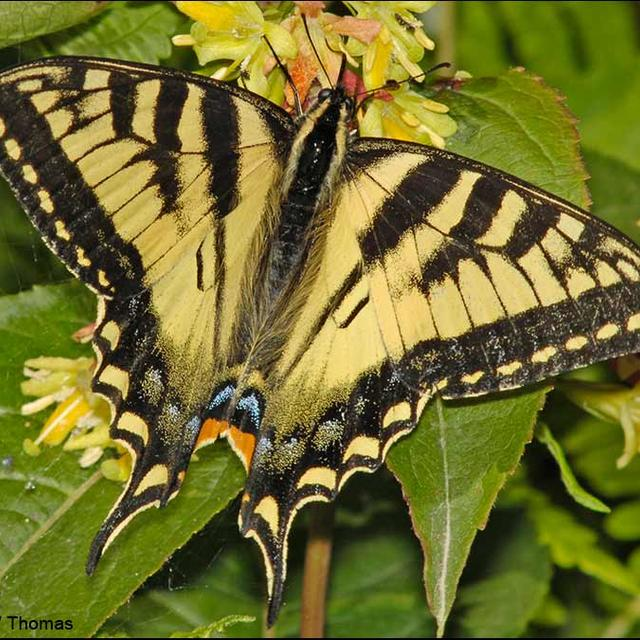
\includegraphics{Papilio_canadensis.png}
\caption{Photo de Papilio canadensis observé dans son habitat
naturel.{}}
\end{figure}

!{[}Répartition de Papilio canadensis au Québec au fil des années.{}{]}
\#ajouter une png ou jpg de notre figure obtenue

Dans cette section, nous analysons l'évolution de la biodiversité des
lépidoptères au fil du temps à travers plusieurs visualisations. Nous
allons créer des cartes et des graphiques pour observer les variations
et tendances.

\subsection{\texorpdfstring{\textbf{Méthodes}}{Méthodes}}\label{muxe9thodes}

\subsubsection{Cartes de biodiveristé
spatio-temporelle}\label{cartes-de-biodiveristuxe9-spatio-temporelle}

Pour l'étude de la biodiversité des Lépidoptère dans le temps et
l'espace, une image regroupant six cartes a été produites. Dans cette
image, on observe la carte de la province du Québec qui est notre air
d'étude principale. Les points géographiques de la base de données qui
sont à l'extérieur de la province ne sont pas pris en compte. La carte
la plus anciennes débute en 1875 et représente les données sur 25 ans,
soit de 1875 jusqu'à la fin de 1879, ces bonds de 25 ans de données vont
jusqu'au données les plus récentes, soit en 2024. Cette image permet
donc de combiner une analyse temporelle (par tranche de 25 ans) et une
agrégation spatiale via une grille hexagonale. En effet, une grille
hexagonable est utilisée pour éviter les effets de bord qu'on a avec une
grilles carrées. De plus, elle permet une meilleure agégration spatiale.
La projection utilisée pour cette carte est EPSG 32198 qui est la
projection locale du Québec. Cela permet une représentation précise à
l'échelle régionale. Pour finir, une moyenne de nombre d'espèces par
cellule pour chaque période de temps a été fait. Ce qui donne une idée
plus stable et comparable de la diversité à travers le temps. En
conclusion, ces 6 cartes sont combinées en une seule image finale, ce
qui permet une comparaison visuelle claire de l'évolution
spatio-temporelle de la diversité spécifique au Québec. Ce qui est utile
visualiser les zones où la diversité augmente, diminue ou reste stable.

\subsection{Visualisation des
données}\label{visualisation-des-donnuxe9es}

Les graphiques ci-dessous montrent l'évolution de la biodiversité des
lépidoptères pour différentes périodes et critères. Nous avons créé six
graphiques pour illustrer les tendances dans les données des
lépidoptères.

\begin{figure}
\centering
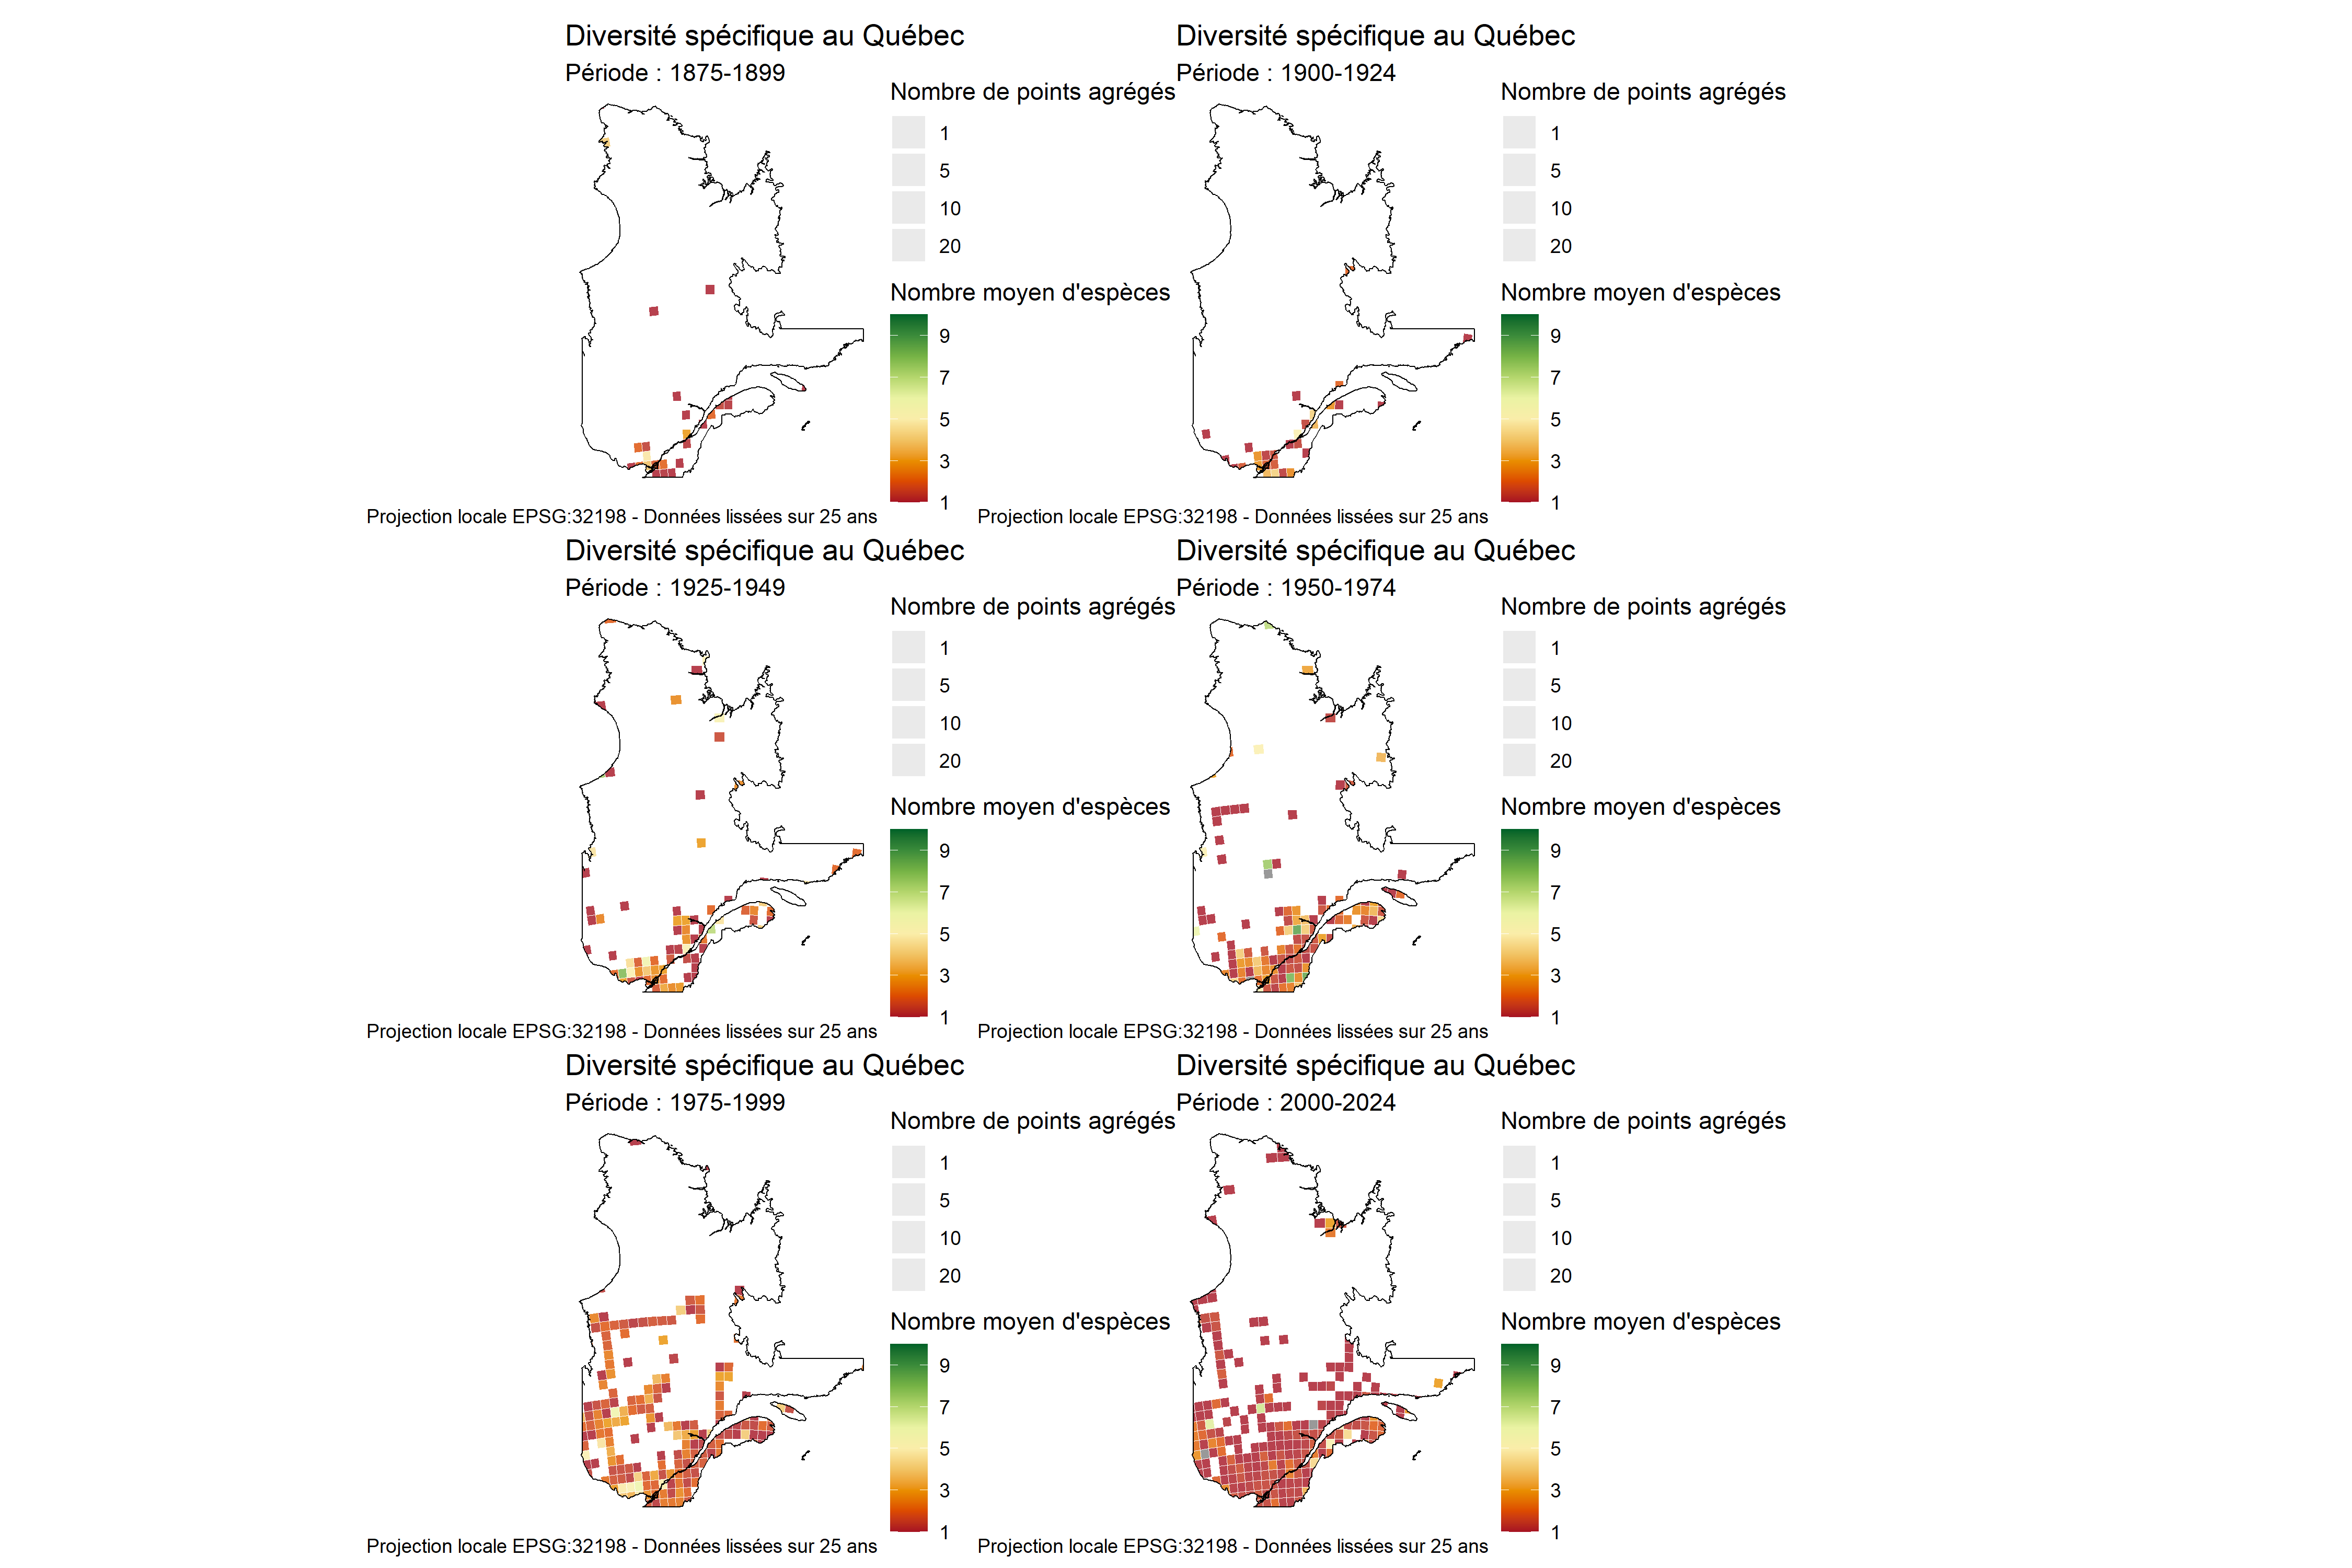
\includegraphics{../Figures_analyse/cartes_combinees.png}
\caption{\emph{Image de la province du Québec et de six cartes qui
montre l'évolution de la biodiversité des espèces de lépidoptères via le
temps avec des fenêtres de 25 ans}}
\end{figure}

\subsection{\texorpdfstring{\textbf{Résultats}}{Résultats}}\label{ruxe9sultats}

\subsubsection{Cartes de biodiveristé
spatio-temporelle}\label{cartes-de-biodiveristuxe9-spatio-temporelle-1}

Ces cartes montrent une augmentation de la couverture spatio-temporelle
des données au fil des décennies. Plus on avance dans le temps, plus il
y a des cellules remplies et plus les données sont denses et complètes.
On voit aussi une légère augmentation du nombre d'espèces dans certaines
régions, mais cette tendance est influencée par autre chose.

Un premier point important a aborder est que entre 1975 et 1899 il y a
très peu de données et celle-ci sont concetrées autour de grandes villes
comme Montréal, Québec, Sherbrooke, etc. La diversité moyenne pour cette
période est faible à modérée, mais les données sont trop rares pour
conclure quelques choses. Si on s'attarde entre 1900-1934 et 1925-1949,
on remarque uen progression lente de la couverture via les données
d'échantillonnage. Il y a encore peu d'échantillons, donc les valeurs de
diveristé sont peu fiables. Les zones urbaines du sud par contre sont
bien couvertes. De 1950-1974, on voit une nette amélioration de la
couverture, des cellules commencent à atteindre une diversité de 7-9
espèces en moyenne dans le sud de la province. Par contre, de 1975-1999,
il y a un essort de données. La majorité du sud du Québec est maintenant
couverte, surtout autour des grands centres et zones garicoles. On
remarque aussi plus de verts ce qui indique une augmentation du nombre
d'espèces osbervées. Pour notre dernière plage de temps, de 2000-2024,
il y a une couverture plus dense et étendue. La diversité moyenne est
plus élevée dans plusieurs régions. Cela est probablement lié à une
explosion des efforts de suivi, l'arrivée de bases de données en ligne
comme iNaturalist.

\subsection{\texorpdfstring{\textbf{Analyse}}{Analyse}}\label{analyse}

\subsubsection{Cartes de biodiveristé
spatio-temporelle}\label{cartes-de-biodiveristuxe9-spatio-temporelle-2}

Un biais de la cartes de biodiversité spatio-temporelle est que plus on
avance dans le temps plus il y a d'osbervation ce qui logique. Par
contre, ces données reflétent aussi les efforts d'échantillonnage autant
que la réalité biologique. Ce qui mène aussi à se poser la question pour
les zones en rouges (faible diveristé) si elles représentent réellement
peu d'espèces ou simlement un manque de points d'échantillonnage. De
plus, le sud du Québec est a plus de données et c'est aussi la qu'on
remarque une augmentation de la diveristé. D'autre part, à partir de
1975, on voit une bonne stabilisation du nombre d'espèces moyen dans
plusieurs cellules, ce qui pourrait refléter un effort d'échantillonnage
suffisant pour capter la vrai diversité locale.

\showmatmethods
\showacknow
\pnasbreak

\phantomsection\label{refs}
\begin{CSLReferences}{0}{1}
\bibitem[\citeproctext]{ref-belkin2002using}
\CSLLeftMargin{1. }%
\CSLRightInline{Belkin M, Niyogi P (2002) Using manifold stucture for
partially labeled classification. \emph{Advances in Neural Information
Processing Systems}, pp 929--936.}

\bibitem[\citeproctext]{ref-berard1994embedding}
\CSLLeftMargin{2. }%
\CSLRightInline{Bérard P, Besson G, Gallot S (1994) Embedding riemannian
manifolds by their heat kernel. \emph{Geometric \& Functional Analysis
GAFA} 4(4):373--398.}

\bibitem[\citeproctext]{ref-coifman2005geometric}
\CSLLeftMargin{3. }%
\CSLRightInline{Coifman RR, et al. (2005) Geometric diffusions as a tool
for harmonic analysis and structure definition of data: Diffusion maps.
\emph{Proceedings of the National Academy of Sciences of the United
States of America} 102(21):7426--7431.}

\end{CSLReferences}



% Bibliography
% \bibliography{pnas-sample}

\end{document}
